\section{香港人都是中國人,為何還要討論身分認同?}

首先,香港人並非全都是中國人。香港是一個國際城市,即使不是中華人民共和國國民的外國人也可以成為香港永久性居民。無論是主觀認同或是客觀定義上,成為中國人也不是成為香港人的必須條件。

香港居民和中國公民是兩個交叉但互不從屬的類別。在香港的中國公民,固然不一定都是香港居民(如大陸遊客),即使是居民也不一定是永久性居民(如持學生或工作簽證);與此同時,身為中國公民也不是成為香港居民或香港永久性居民的必要前設。香港有數十萬的外籍人口居留甚至定居,例如不少南亞少數族裔就是連續幾代人都在香港生活,卻沒有入籍成為中國公民,拿的仍然是南亞各國的護照。這兒還未談到香港有數以十萬計擁有外國護照的回流人士,他們按中國《國籍法》已因取得外國國籍和在外國定居而失去中國國籍,但他們仍然是香港永久性居民。只要他們重新定居香港,均可以享有各種永久性居民的待遇,也可以在各級選舉當中投票。即使《基本法》第六十七條也尊重這個客觀現實,容許一定比例的非中國公民和持外國居留權人士成為立法會議員。

說起《基本法》,條文列明不論永久性居民或非永久性居民都是香港居民。誰是非永久性居民呢?數以十萬計來自菲律賓和印尼等國的外籍家務工就是一例。他們不少在香港服務多年,和香港人一起生活,通過家務勞動來釋放本來未能外出工作的勞動力,撐起香港的經濟。廣義來說,他們也是香港人。這個討論重要,因為香港是一個國際城市,任何假定香港人都是中國人的說法一旦成為公共政策,就會構成嚴重的執行問題。例如政府極其量只可鼓勵香港人多了解中國國情,卻不可能要求所有香港人都要學習愛國,因為那些外國回流的華裔和在港定居的少數族裔一定會反問,政府是否要他們背叛加拿大或者巴基斯坦?

\begin{figure}[htbp]
    \centering
    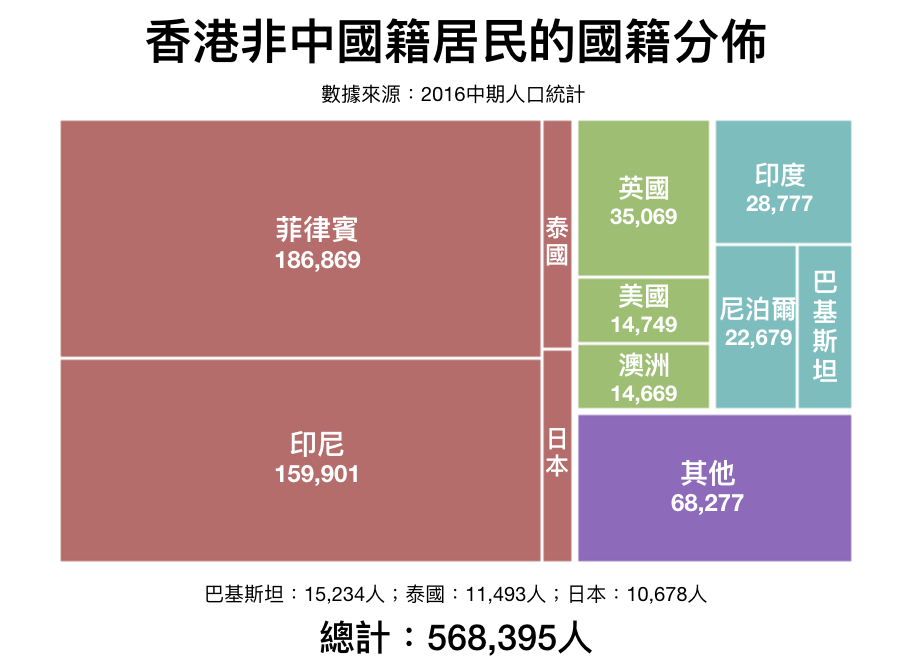
\includegraphics[width=0.7\textwidth]{c11/h-klesson1-015.png}
    \caption{香港居民中有不少並非持有中國國籍} 
\end{figure}

我們也可從國籍問題點出坊間不少對國民身分的誤解。儘管國籍可通過血緣關係獲得,但兩者本身不一定對等,所以和國籍相關的一系列政治權責期望,也不應基於血緣簡單推斷。國籍本身歸根究底是一個社會產物,既按當時當地社會定義,也可按個人情況取得或撤銷。因此,任何以「同文同種」的說法為基礎,假定某個體或社群必然要接受某些政治權責期望,無論是對國家或政權的效忠,本身也是十分不嚴謹的。事實上,中華人民共和國是個多民族國家,漢族只是其中一員。有香港政治人物曾經說過新年收紅包就該自認中國人,正正是犯了此等謬誤。畢竟,中華人民共和國境內有不少沒有封紅包甚至沒有過農曆新年傳統的民族;相反,東亞各國各民族和眾多海外華人都有封紅包的習慣,但他們都不是中華人民共和國國民。

國籍尚且如此,個人認同則更為複雜。說起來,孫中山搞革命的時候還拿過美國護照,曾經一度持有雙重國籍,但據稱只是為了方便行走江湖,恐怕他對美國的身分認同十分有限。反過來說,許多香港人本來沒有選擇要有中國國籍,而是後來被賦予的。他們覺不覺得自己是中國人,又或覺得自己是怎樣的中國人,當然也是可以討論的。

按香港大學的民意調查所得,香港人的中國身分認同在九七後本來是上升的。調查顯示在一九九七年八月,共有19\%的受訪者認為自己是香港人;到了二零零八年六月,也就是汶川地震和北京奧運期間,比例上升至39\%,上升超過一倍。按香港中文大學亞太研究所的調查,受訪的逾千名香港市民當中超八成都說自己已捐款支持汶川賑災,很難說是對中國完全抗拒的表現。

不過,數據從此調頭向下,抗拒情緒特別在年輕人之間十分普遍。很多過去沒有被質疑的「愛國」表現,都受到各種挑戰和重新檢視。例如港府出資一百億的各個四川重建項目當中,援建綿陽的中學在未得港方同意下被私自拆除變成豪華商場,就在香港引起公眾嘩然。到了二零一三年的雅安地震,港府再向立法會申請撥款賑災,就招來社會輿論反對。到了二零一七年年底,整體認同自己是中國人的只有15\%,而十八至二十九歲的受訪者當中更只有0.3\%認為自己是中國人。

\begin{figure}[htbp]
    \centering
    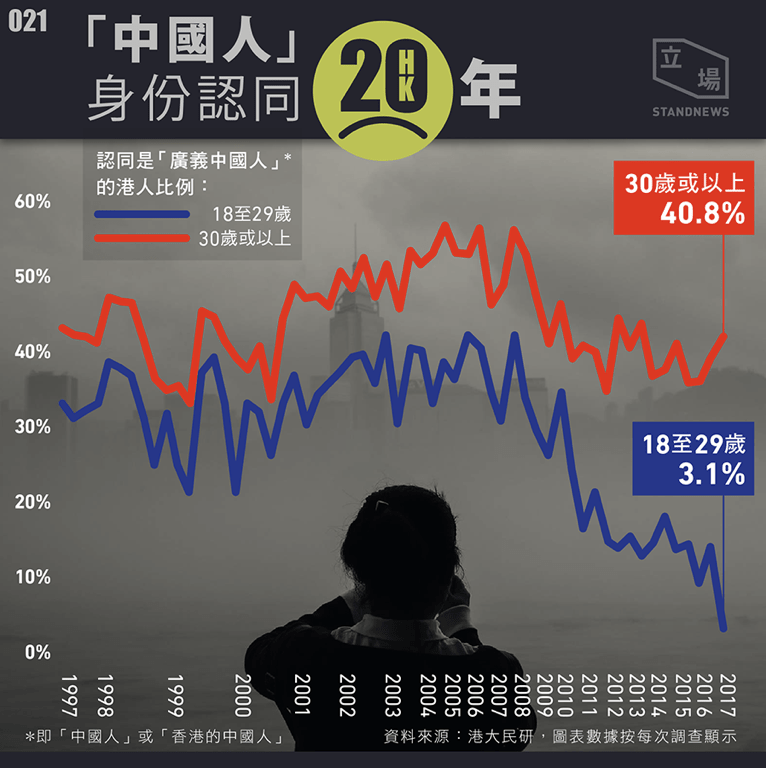
\includegraphics[width=0.7\textwidth]{c11/h-klesson1-016.png}
    \caption{特區成立後的香港身分認同改變。對中國人的認同程度在2017年中後進一步下跌。} 
\end{figure}

這些改變和前文提到香港在九七前後經歷的社會變遷有密切關係。對於九七前成長的香港人,中國往往以三種形式出現。第一,是他們自己或上一代的故鄉。他們很可能有回鄉探親的經歷,曾經挑著裝滿舊衣和雜糧的「紅白藍大膠袋」長途跋涉的去接濟八十年代初仍活在貧困之中的同鄉親戚。第二,是教課書中的古典中國。普遍香港學生都會通過中學教育學會最基本的中國文學和中國歷史,能夠背誦「出師表」和「兵車行」等的文言作品,並從李白所寫的詩詞中猜想「長江天際流」的景致。第三,是改革開放早期香港人北上設廠、消費以至尋歡的冒險樂園。曾幾何時,深圳別名就是「心震」,既代表混亂也代表機會。都市傳說聲稱在酒店一覺醒來會發現腎藏已被割掉,夜店大火死傷無數則是現實新聞。這三個中國當然都是片面的,卻都是九七前香港人的重要情感標記。在這些想像當中,香港人可以是某種意義下的中國人,儘管這個「中國人」的身分明顯和中華人民共和國國民有所區別。

換言之,在九七前的香港,即使沒有政治學訓練的香港人也會明白「國家」、「政權」與「民族」是三個概念,之間的同異是可以坐下來慢慢談的。然而這些區別和討論空間在九七後卻逐漸消失。在國家認同的號召下,要做中國人就要做中華人民共和國國民,也就要接受中共政權。事實上,中國政府時刻都在干擾香港的高度自治(見問題十六),成為許多香港管治問題無法解決的根本原由。在這樣的政治環境下,繼續把中國認同寄託於壯麗山河或文化情懷當中,已顯得越來越蒼白無力。特別是九七後成長的新一代,他們還未有機會如上一代那樣培養中國想像,也沒有經歷過九七前對未來的恐懼和期待,就要面對中共政權主導香港政治的客觀事實,所以反抗情緒比九七前成長的一代反而來得更直接:如果當中國人就等於接受被中共統治,那麼他們寧願不做中國人。

九七前後的分別也打破了另一個中國大陸對於香港身分認同的錯誤理解。在中國大陸的主流論述中,香港人對中國認同的抗拒是因為受英國殖民統治太久,被英殖教育所蒙蔽,對中國大陸認識不足,所以要通過再教育來學習如何做好一個中國人。事實上在英國殖民統治下成長的香港人對中國認同並不反感,抗拒的是中共政權;在九七後長大沒有受過英殖教育的年輕人,反而對中國認同更為反感。此外,也有調查顯示年輕人對中國大陸認識不淺,例如有95%受訪者曾到中國大陸,85%能閱讀簡體字,46%每月多次或每天使用中國大陸網站,可見他們對中國認同的抗拒不能單純以認識不足來解釋。

雖然九七後香港已成為中華人民共和國的一部分,但不代表香港人的身分認同就會再無爭議。討論身分認同,可以幫助我們認清社會變遷。而當政府制訂公共政策時不理會這些爭議,或對其的現況或原由有錯誤判斷,更會造成不必要的社會矛盾。



伸延閱讀:

張勇,陳玉田(2002):《香港居民的國籍問題》,三聯書店(香港)有限公司。

馬傑偉(2008):〈從「現代香港」到「民主香港」的漫長過程〉,本土論述編輯委員會、新力量網絡編《本土論述 2008》,香港:上書局。

網上資源:

\href{https://thestandnews.com/politics/圖析香港主權移交20年/}{圖析新聞(2017):〈圖析香港主權移交20年〉:立場新聞,2017年6月30日}